\documentclass{ctexart}
\usepackage{EC}
\begin{document}
\section{硼及其化合物}
\subsection{单质硼和金属硼化物}
由于单质硼和硼化物(尤其是和金属形成的硼化物)的结构比较类似,因此我们在此处一起介绍.
\subsubsection{单质硼的制备}
通过还原含硼化合物的方法可以方便地制备得到\ce{B}单质.
\begin{center}
    \ce{3Mg + B2O3 -> 3MgO + 2B}\\
    \ce{2KBF4 + 6KCl ->T[熔融\ce{KCl/KF}][电解] 8KF + 2B + 3Cl2}\\
    \ce{2BBr3 + 3H2 -> 2B + 6HBr}\\
    \ce{B_nH_m ->T[加热] n B + $\dfrac{m}{2}$ H2}
\end{center}
通常得到的硼是无定形的,但是改变温度条件也可以得到各种晶型的硼单质.
\subsubsection{单质硼的结构}
各种单质硼都具有相当复杂的结构,这主要是\ce{B}本身的缺电子结构使其的成键较为复杂所致.不过,一般而言,各种单质硼总是由\ce{\{B12\}}多面体衍生而来.
\paragraph{正十二面体与正二十面体的画法}
清晰地表示复杂簇合物的立体结构是你应当掌握的技巧.我们在这里介绍两种最典型的高对称性多面体的画法.
\subparagraph{正十二面体的画法}
我们可以按照以下步骤绘制正十二面体.
\begin{enumerate}[label=$\mathit{Step\ \arabic*.}$,topsep=0pt,parsep=0pt,itemsep=0pt,partopsep=0pt,leftmargin=*]
    \item 画一个正五边形.
    \item 画一个相对步骤$\mathit{1}$中旋转$180^\circ$的大小相同的正五边形,注意透视关系.
    \item 沿步骤$\mathit{1}$和步骤$\mathit{2}$中的两个正五边形的所有$10$条外角平分线方向画出等长的线段.
    \item 顺次连接步骤$\mathit{3}$中产生的各个外围顶点.
\end{enumerate}
\begin{figure}[H]
    \centering
    \subfigure[$\mathit{Step\ 1.}$]{
        \begin{minipage}[b]{.23\linewidth}
            \centering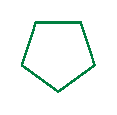
\includegraphics{picture/12-1.eps}
        \end{minipage}
    }
    \subfigure[$\mathit{Step\ 2.}$]{
        \begin{minipage}[b]{.23\linewidth}
            \centering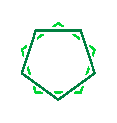
\includegraphics{picture/12-2.eps}
        \end{minipage}
    }
    \subfigure[$\mathit{Step\ 3.}$]{
        \begin{minipage}[b]{.23\linewidth}
            \centering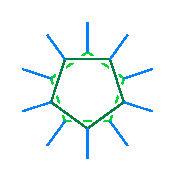
\includegraphics{picture/12-3.eps}
        \end{minipage}
    }
    \subfigure[$\mathit{Step\ 4.}$]{
        \begin{minipage}[b]{.23\linewidth}
            \centering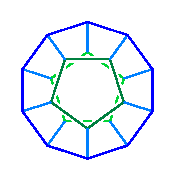
\includegraphics{picture/12-4.eps}
        \end{minipage}
    }
    \caption{正十二面体的画法}
\end{figure}
\subparagraph{正二十面体的画法}
我们可以按照以下步骤绘制正二十面体.
\begin{enumerate}[label=$\mathit{Step\ \arabic*.}$,topsep=0pt,parsep=0pt,itemsep=0pt,partopsep=0pt,leftmargin=*]
    \item 画一个正三角形(记为$\triangle{A}$).
    \item 画一个相对步骤$\mathit{1}$中旋转$180^\circ$的大小相同的正三角形(记为$\triangle{B}$),注意透视关系.
    \item 沿$\triangle{A}$和$\triangle{B}$的所有$6$条外角平分线画出等长的线段.
    \item 将$\triangle{B}$形成的外围顶点与$\triangle{A}$的顶点依次连接.
    \item 将$\triangle{A}$形成的外围顶点与$\triangle{B}$的顶点依次连接,注意透视关系.
    \item 顺次连接步骤$\mathit{3}$中产生的各个外围顶点.
\end{enumerate}
\begin{figure}[H]
    \centering
    \subfigure[$\mathit{Step\ 1.}$]{
        \begin{minipage}[b]{.3\linewidth}
            \centering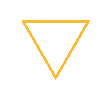
\includegraphics{picture/20-1.eps}
        \end{minipage}
    }
    \subfigure[$\mathit{Step\ 2.}$]{
        \begin{minipage}[b]{.3\linewidth}
            \centering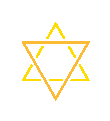
\includegraphics{picture/20-2.eps}
        \end{minipage}
    }
    \subfigure[$\mathit{Step\ 3.}$]{
        \begin{minipage}[b]{.3\linewidth}
            \centering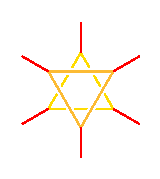
\includegraphics{picture/20-3.eps}
        \end{minipage}
    }
    \subfigure[$\mathit{Step\ 4.}$]{
        \begin{minipage}[b]{.3\linewidth}
            \centering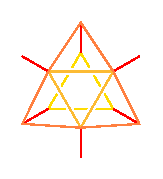
\includegraphics{picture/20-4.eps}
        \end{minipage}
    }
    \subfigure[$\mathit{Step\ 5.}$]{
        \begin{minipage}[b]{.3\linewidth}
            \centering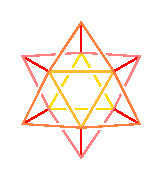
\includegraphics{picture/20-5.eps}
        \end{minipage}
    }
    \subfigure[$\mathit{Step\ 6.}$]{
        \begin{minipage}[b]{.3\linewidth}
            \centering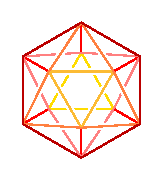
\includegraphics{picture/20-6.eps}
        \end{minipage}
    }
    \caption{正二十面体的画法}
\end{figure}
\paragraph{硼的同素异形体}
我们主要(简单地)介绍以下几种硼的同素异形体.
\begin{enumerate}[label=\tbf{\arabic*.},topsep=0pt,parsep=0pt,itemsep=0pt,partopsep=0pt]
    \item $\alpha$-三方硼\\
        $\alpha$-三方硼是硼最简单的同素异形体.它由近似立方密堆积的\ce{B12}二十面体组成,因而退化成R心六方点阵.
        \begin{figure}[H]
            \centering
            \subfigure[$\alpha$-三方硼的晶胞示意图]{
                \begin{minipage}[b]{.48\linewidth}
                    \centering\includegraphics[scale=0.1]{picture/alpha-B.eps}
                \end{minipage}
            }
            \subfigure[$\alpha$-三方硼沿$\mbf{a}+\mbf{b}$方向的投影图]{
                \begin{minipage}[b]{.48\linewidth}
                    \centering\includegraphics[scale=0.1]{picture/alpha-B-2.eps}
                \end{minipage}
            }
            \caption{$\alpha$-三方硼的晶体结构}
        \end{figure}
    \item $\beta$-三方硼\\
        $\beta$-三方硼是硼在热力学上最稳定的同素异形体.它的结构则要复杂得多.\\
        $\beta$-三方硼的晶胞中有$105$个\ce{B}原子.其中的\ce{B84}单元是由\ce{B12}二十面体以及每个\ce{B}相连的\ce{B6}单元组成.\ce{B6}单元是向外的五角锥形,与正二十面体的一部分几乎一致.\ce{B84}单元之间由\ce{B10}半二十面体(注意其结构类似二十面体的一部分)以及额外的一个\ce{B}原子连接,比例为$1:2:1$,因此结构基元总计有$105$个\ce{B}原子.
        \begin{figure}[H]
            \centering
            \subfigure[\ce{B84}单元的结构示意图]{
                \begin{minipage}[b]{.48\linewidth}
                    \centering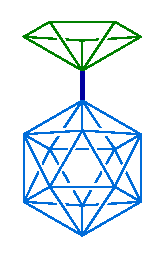
\includegraphics{picture/B84.eps}
                \end{minipage}
            }
            \subfigure[\ce{B10}单元的结构示意图]{
                \begin{minipage}[b]{.48\linewidth}
                    \centering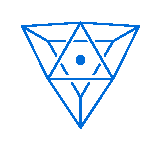
\includegraphics{picture/B10.eps}
                \end{minipage}
            }
            \caption{$\beta$-三方硼的结构示意图}
        \end{figure}
        至于整体的晶胞,因为太过复杂,故此处不单独展示.如果你有兴趣,可以自行查阅其晶胞\footnote{恕笔者直言,长得有点奇行种.}.
    \item 其它硼的同素异形体\\
        总而言之,其它硼的同素异形体,例如$\beta$-四方硼,$\gamma$-硼的结构都与上述两者有类似之处,都是由\ce{B12}二十面体及其衍生结构组成的.它们的晶胞也比较复杂,你可以自行查阅之.
\end{enumerate}
\subsubsection{金属硼化物的制备}
制备金属硼化物主要有以下几种方法.
\begin{enumerate}[label=\tbf{\arabic*.},topsep=0pt,parsep=0pt,itemsep=0pt,partopsep=0pt]
    \item 直接由单质直接化合.例如:
        \begin{center}
            \ce{Cr + n B ->T[$1150\tc$] CrB_n}
        \end{center}
    \item 用硼单质还原金属氧化物(这种办法比较浪费难得的硼单质).例如:
        \begin{center}
            \ce{Sc2O3 + 7B ->T[$1800\tc$] 2ScB2 + 3BO}
        \end{center}
        这里需要注意的是\ce{B}单质和\ce{B2O3}大约在$1350\tc$时反应生成玻璃状的\ce{(BO)_n}聚合物.
    \item 用\ce{H2}还原金属和硼的卤化物混合物,或用碳还原金属和硼的氧化物混合物,或用硼碳化物还原金属氧化物.例如:
        \begin{center}
            \ce{2TiCl4 + 4BCl3 + 10H2 ->T[$1300\tc$] 2TiB2 + 20HCl}\\
            \ce{V2O5 + B2O3 + 8C ->T[$1500\tc$] 2VB + 8CO}\\
            \ce{Eu2O3 + 3B4C ->T[$1600\tc$] 2EuB6 + 3CO}\\
            \ce{7Ti + B2O3 + 3B4C ->T[$2000\tc$] 7TiB2 + 3CO}
        \end{center}
    \item 熔融盐的电解沉积.将金属氧化物和\ce{B2O3}混合熔融于合适的盐中,然后用石墨电极电解即可在阴极得到硼化物.
\end{enumerate}
\subsubsection{金属硼化物的结构}
\paragraph{富金属的金属硼化物}
这类物质的通式为\ce{M_n B},其中\ce{M}为金属元素并且(大致而言)$n\geqslant0.5$.通常而言,硼原子总是处于三棱柱(或者加数个帽)的配位环境中,并且随着$n$变小时,\ce{B}还会从分立转为线形的\ce{B2},链状或平面的\ce{B_n}等形式.\\
\indent 这里给出一些简单的例子以供参考.
\begin{figure}[H]
    \centering
    \subfigure[\ce{MgB2}的晶胞示意图]{
        \begin{minipage}[b]{.48\linewidth}
            \centering\includegraphics[scale=0.1]{picture/MgB2-1.eps}
        \end{minipage}
    }
    \subfigure[\ce{MgB2}的$c$轴投影图]{
        \begin{minipage}[b]{.48\linewidth}
            \centering\includegraphics[scale=0.1]{picture/MgB2-2.eps}
        \end{minipage}
    }
    \caption{\ce{MgB2}的晶体结构}
\end{figure}
\begin{figure}[H]
    \centering
    \subfigure[\ce{ReB3}的晶胞示意图]{
        \begin{minipage}[b]{.48\linewidth}
            \centering\includegraphics[scale=0.1]{picture/Re3B-1.eps}
        \end{minipage}
    }
    \subfigure[\ce{ReB3}的晶胞示意图]{
        \begin{minipage}[b]{.48\linewidth}
            \centering\includegraphics[scale=0.1]{picture/Re3B-2.eps}
        \end{minipage}
    }
    \caption{\ce{ReB3}的晶体结构}
\end{figure}
\paragraph{富硼的金属硼化物}
富硼的金属硼化物,从\ce{MB4}到\ce{MB66}等等,大多以\ce{B}的团簇和填充其中的金属原子组成.我们现在选取主要的几种进行介绍.
\begin{enumerate}[label=\tbf{\arabic*.},topsep=0pt,parsep=0pt,itemsep=0pt,partopsep=0pt]
    \item \tbf{\ce{MB4}}\\
        典型的如四方晶系的\ce{ThB4},其中含有\ce{B6}八面体结构,并由线形的\ce{B2}在层内将其相连;\ce{Th}原子则填充在它们形成的$c$轴方向的空隙中.对于\ce{B2}单元中的\ce{B}原子,仍然被\ce{Th}原子六配位.这可以视作\ce{MB2}和\ce{MB6}结构中间的过渡.
        \begin{figure}[H]
            \centering
            \subfigure[\ce{ThB4}的晶胞示意图]{
                \begin{minipage}[b]{.48\linewidth}
                    \centering\includegraphics[scale=0.1]{picture/ThB4-1.eps}
                \end{minipage}
            }
            \subfigure[\ce{ThB4}的晶胞示意图]{
                \begin{minipage}[b]{.48\linewidth}
                    \centering\includegraphics[scale=0.1]{picture/ThB4-2.eps}
                \end{minipage}
            }
            \caption{\ce{ThB4}的晶体结构}
        \end{figure}
    \item \tbf{\ce{B4C}}\\
        确切的验证表明实际上组成为\ce{B13C2},但是也可以在\ce{B13C2}到\ce{B12C3}(即\ce{B4C})的范围内变动.\ce{B13C2}的晶体结构如下所示.
        \begin{figure}[H]
            \centering
            \subfigure[\ce{B13C2}的晶胞示意图]{
                \begin{minipage}[b]{.48\linewidth}
                    \centering\includegraphics[scale=0.1]{picture/B13C2-1.eps}
                \end{minipage}
            }
            \subfigure[\ce{B13C2}的晶胞示意图]{
                \begin{minipage}[b]{.48\linewidth}
                    \centering\includegraphics[scale=0.1]{picture/B13C2-2.eps}
                \end{minipage}
            }
            \caption{\ce{B13C2}的晶体结构}
        \end{figure}
        \indent 这种三方晶系的晶体可以视作线形\ce{CBC}单元做立方密堆积,\ce{B12}单元填入所有八面体空隙中而形成的.把\ce{CBC}单元中的\ce{B}也(部分地)换成\ce{C},就可以得到组成逐渐接近\ce{B4C}的物质.
    \item \tbf{\ce{MB6}}\\
        典型的如立方晶系的\ce{LaB6}.其中的\ce{B6}八面体单元按简单立方堆积形成网状结构,\ce{La}则填入所有立方体空隙中.因此,\ce{La}原子的配位数为$24$,配位多面体为截角立方体,每个与其相邻的\ce{B6}八面体贡献一个三角形面.
        \begin{figure}[H]
            \centering
            \subfigure[\ce{LaB6}的晶胞示意图]{
                \begin{minipage}[b]{.48\linewidth}
                    \centering\includegraphics[scale=0.1]{picture/LaB6-1.eps}
                \end{minipage}
            }
            \subfigure[\ce{LaB6}的八倍晶胞示意图]{
                \begin{minipage}[b]{.48\linewidth}
                    \centering\includegraphics[scale=0.1]{picture/LaB6-2.eps}
                \end{minipage}
            }
            \subfigure[\ce{LaB6}中\ce{La}的配位多面体]{
                \begin{minipage}[b]{.9\linewidth}
                    \centering\includegraphics[scale=0.1]{picture/LaB6-3.eps}
                \end{minipage}
            }
            \caption{\ce{LaB6}的晶体结构}
        \end{figure}
    \item \tbf{\ce{MB12}}\\
        典型的如立方晶系的\ce{UB12}.其中的\ce{B12}单元并不是常见的正二十面体,而是立方八面体.你可以将立方体的棱心依次连接而得到它的形状.\\
        在\ce{UB12}中,\ce{B12}立方八面体做立方密堆积,\ce{U}原子填入所有八面体空隙.其中的\ce{U}原子也是$24$配位的,但配位形式是截角八面体,每个与其相邻的\ce{B12}单元贡献一个正方形面.\\
        顺带一提,此时\ce{B12}单元形成的四面体空隙是一个截角四面体,每个\ce{B12}立方八面体贡献一个三角形面.
        \begin{figure}[H]
            \centering
            \subfigure[\ce{UB12}的晶胞示意图]{
                \begin{minipage}[b]{.48\linewidth}
                    \centering\includegraphics[scale=0.1]{picture/UB12-1.eps}
                \end{minipage}
            }
            \subfigure[\ce{UB12}晶胞的$a$轴投影图]{
                \begin{minipage}[b]{.48\linewidth}
                    \centering\includegraphics[scale=0.1]{picture/UB12-2.eps}
                \end{minipage}
            }
            \caption{\ce{UB12}的晶体结构}
        \end{figure}
\end{enumerate}
\subsection{硼烷及其衍生物}
\subsubsection{Wade规则}
\paragraph{Wade规则介绍}
多面体骨架电子对理论(Polyhedral Skeletal Electron Pair Theory, PSEPT)试图从多面体骨架的几何形状和电子数之间的关系上来阐明金属原子簇的结构规律.这一规则最初由Kenneth Wade制定,因此又被称为Wade规则.\\
\indent 我们现在来介绍Wade规则的具体内容.\\
\indent $\mathit{Step\ 1.}$\ \tbf{确定骨架原子数}\\
\indent 骨架原子通常是IVA族及之前的元素或过渡金属元素,而\ce{N,O}等元素则应当作为额外的配体考虑.这样就能确定骨架原子数$n$.\\
\indent $\mathit{Step\ 2.}$\ \tbf{确定骨架电子数}\\
\indent 每个骨架原子都拿出三个价轨道参与骨架的成键,剩余的价轨道一般对应端基原子且需要填满.在满足端基的情况下,骨架原子剩余的电子参与成键,将计入骨架电子数.\\
\indent 例如,对于硼烷而言,骨架\ce{B}原子有四个价轨道,除去三个用于构成骨架之外剩余一个与端基\ce{H}相连,端基\ce{B-H}键需用去\ce{B}的一个价电子,因而剩余$2$个电子计入骨架电子数.类似地,对于碳硼烷中的\ce{CH}基团而言,将有$3$个电子计入骨架电子数.\\
\indent 对于过渡金属\ce{M}的羰基簇合物而言,\ce{M}有九个价轨道,除去三个用于构成骨架之外剩余六个价轨道.假设其价电子数为$v$,端基配位的基团提供的总电子数为$w$,那么充满六个价轨道后计入骨架电子的数目为$v+w-12$.下面是一些典型的过渡金属碎片提供的骨架电子数.
\begin{table}[H]
    \centering
    \begin{tabular}{c|c|c|c|c|c}
        \hline
        $v$ &过渡金属\ce{M} &\ce{M(CO)2}$(w=4)$ &\ce{M(Cp)}$(w=5)$  &\ce{M(CO)3}$(w=6)$ &\ce{M(CO)4}$(w=8)$ \\\hline
        $6$ &\ce{Cr,Mo,W}   &$-$    &$-1$   &$0$    &$2$ \\
        $7$ &\ce{Mn,Tc,Re}   &$-1$    &$0$   &$1$    &$3$ \\
        $8$ &\ce{Fe,Ru,Os}   &$0$    &$1$   &$2$    &$4$ \\
        $9$ &\ce{Co,Rh,Ir}   &$1$    &$2$   &$3$    &$-$ \\
        $10$ &\ce{Ni,Pd,Pt}   &$2$    &$3$   &$-$    &$-$ \\\hline
    \end{tabular}
    \caption{过渡金属碎片提供的骨架电子数}
\end{table}
从这里可以看出,\ce{Fe(CO)3}等基团提供的电子数与\ce{BH}相同,\ce{Co(CO)3}等基团提供的电子数与\ce{CH}相同.事实上,在大部分化合物中,这些基团可以相互替换,表现出了相似的性质.这就是\tbf{等瓣相似原理}.\\
\indent 除此之外,尚有不是端基的一些配体.它们通常作为桥连配体或存在于骨架内部,依照不同的配位方式提供不同的电子数目,并全部计入骨架电子数目中.例如,\ce{H}原子计$1$个电子,\ce{CO}配体计$2$个电子,边桥基的\ce{O}原子计$2$个电子,面桥基和体内则分别计$4$个和$6$个电子,等等.\\
\indent 最后,如果我们考虑的对象是离子,应将电荷也计入骨架电子中.\\
\indent 按照以上的步骤,我们就能得出骨架电子数$m$.\\
\indent $\mathit{Step\ 3.}$\ \tbf{确定骨架的结构}\\
\indent Wade发现$m$和$n$之间的关系决定了簇合物的立体结构.简单而言,\tbf{簇合物是由$m-n-2$个顶点的闭式多面体去掉$m-2n-2$个顶点形成的多面体}.\\
\indent 上面这句话听起来很拗口.我们首先来解决第一个问题:闭式多面体的定义.简而言之,闭式多面体是全部由三角形面构成的闭合的多面体.具有$N$个顶点的闭式多面体展示如下.
\begin{figure}[H]
    \centering
    \subfigure[$N=4$\ 正四面体]{\begin{minipage}[b]{.3\linewidth}\centering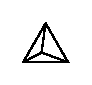
\includegraphics{picture/closo-4.eps}\end{minipage}}
    \subfigure[$N=5$\ 三角双锥]{\begin{minipage}[b]{.3\linewidth}\centering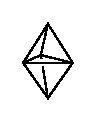
\includegraphics{picture/closo-5.eps}\end{minipage}}
    \subfigure[$N=6$\ 正八面体]{\begin{minipage}[b]{.3\linewidth}\centering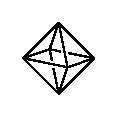
\includegraphics{picture/closo-6.eps}\end{minipage}}
    \subfigure[$N=7$\ 五角双锥]{\begin{minipage}[b]{.3\linewidth}\centering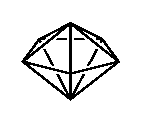
\includegraphics{picture/closo-7.eps}\end{minipage}}
    \subfigure[$N=8$\ 三角十二面体]{\begin{minipage}[b]{.3\linewidth}\centering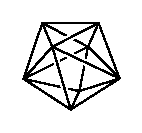
\includegraphics{picture/closo-8.eps}\end{minipage}}
    \subfigure[$N=9$\ 三帽三棱柱]{\begin{minipage}[b]{.3\linewidth}\centering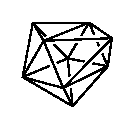
\includegraphics{picture/closo-9.eps}\end{minipage}}
    \subfigure[$N=10$\ 双帽四方反棱柱]{\begin{minipage}[b]{.3\linewidth}\centering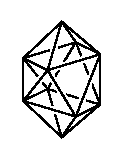
\includegraphics{picture/closo-10.eps}\end{minipage}}
    \subfigure[$N=11$\ 边收缩二十面体]{\begin{minipage}[b]{.3\linewidth}\centering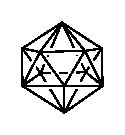
\includegraphics{picture/closo-11.eps}\end{minipage}}
    \subfigure[$N=12$\ 正二十面体]{\begin{minipage}[b]{.3\linewidth}\centering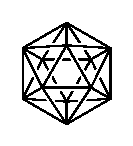
\includegraphics{picture/closo-12.eps}\end{minipage}}
    \caption{具有$N$个顶点的闭式多面体}
\end{figure}
现在,我们按照去除顶点的个数对簇合物分类.
\begin{table}[H]
    \centering\begin{tabular}{|c|c|c|c|}
        \hline
        $m$的取值   &中文名称   &拉丁文名称 &形状\\\hline
        $2n-2$  &双帽闭式   &Bicapped\ $\mathit{closo}$ & 双加帽的具有$n-2$个顶点的闭式多面体 \\\hline
        $2n$  &单帽闭式   &Capped\ $\mathit{closo}$ & 加帽的具有$n-1$个顶点的闭式多面体 \\\hline
        $2n+2$  &闭式   &$\mathit{closo}$ & 具有$n$个顶点的闭式多面体 \\\hline
        $2n+4$  &巢式   &$\mathit{nido}$ & 具有$n+1$个顶点的闭式多面体去除$1$个顶点 \\\hline
        $2n+6$  &蛛网式   &$\mathit{arachno}$ & 具有$n+2$个顶点的闭式多面体去除$3$个顶点 \\\hline
        $2n+8$  &开式   &$\mathit{hypho}$ & 具有$n+3$个顶点的闭式多面体去除$3$个顶点 \\\hline
    \end{tabular}
    \caption{簇合物骨架形状与$m$和$n$的关系}
\end{table}
下面这张图给出了典型的结构\footnote{限于排版原因,请将讲义顺时针旋转$90^\circ$后查阅此图.}.
\begin{figure}[H]
    \centering\includegraphics[scale=0.06,angle=90]{picture/Wade.eps}\caption{Wade规则所预测的多面体形状}
\end{figure}
\indent $\mathit{Step\ 4.}$\ \tbf{确定非端基配体的位置}\\
\indent 实际上端基配体的位置是比较难以确定的.很多配体的不同配位形式所提供的电子数目一致.因此,在没有额外条件下,你可以尽量猜测研究对象具有较高的对称性.
\paragraph{Wade规则的简单应用}
我们在本节举几个简单的例子来说明Wade规则如何应用.\\
$\mathit{Example\ 2.}$\ \ce{[B6H6]^2-}\\
\indent 骨架原子数$n=6$,骨架电子数$m=6\times2+2=14$,因此$m=2n+2$,采取顶点数$N=6$的正八面体结构,无需增删顶点.
\chemfig{B6H62-}{1}{\ce{[B6H6]^2-}的结构}
类似地,你可以知道\ce{[B_n H_n]^2-}的结构就是顶点数$N=n$的闭式多面体.\\
$\mathit{Example\ 1.}$\ \ce{B10C2H12}\\
\indent 骨架原子数$n=12$,骨架电子数$m=10\times2+2\times3=26$,因此$m=2n+2$,采取顶点数$N=12$的正二十面体结构,无需增删顶点.由于\ce{C}原子相对位置的不同,\ce{B10C2H12}事实上有三种异构体.
\begin{figure}[H]
    \centering
    \subfigure[$o$-\ce{B10C2H12}]{
        \begin{minipage}[b]{.3\linewidth}
            \centering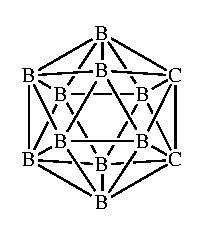
\includegraphics{picture/B10C2H12-o.eps}
        \end{minipage}
    }
    \subfigure[$m$-\ce{B10C2H12}]{
        \begin{minipage}[b]{.3\linewidth}
            \centering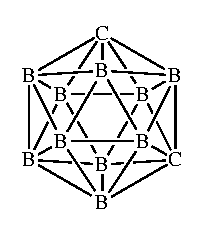
\includegraphics{picture/B10C2H12-m.eps}
        \end{minipage}
    }
    \subfigure[$p$-\ce{B10C2H12}]{
        \begin{minipage}[b]{.3\linewidth}
            \centering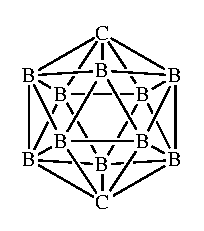
\includegraphics{picture/B10C2H12-p.eps}
        \end{minipage}
    }
\end{figure}
\end{document}